\documentclass[msc]{mestrado}

\usepackage{master}

%% Inicio do documento
\begin{document}
\mainmatter

\headsep=40pt
\oddsidemargin=15pt
% \begin{spacing}{1.4}
\parskip=4pt

%\singlespacing
%\onehalfspacing
%\doublespacing
\setstretch{1.4}

%\chapter{Introdu��o}

%\chapter{Ethernet e Tempo Real}
\label{cap:motivacao} \label{sec:sisHibrid} \label{sec:TempraVTPE}   \label{fig:ethernetFrame} 

%\chapter{O Protocolo \doris{}} % (10 pag)
%\label{cap:doris}
\chapter{\doris: Especifica��o e verifica��o}
\label{cap:doris}

\section{Introdu��o}
\label{sec:intro}

Neste cap�tulo,  um novo protocolo de comunica��o de tempo real, baseado em  Ethernet
compartilhado, � apresentado atrav�s das sua especifica��o formal na linguagem TLA+
\cite{Lamport02a}.

O protocolo \doris, cujo significado em ingl�s � \emph{An Ethernet
  \underline{Do}uble \underline{Ri}ng \underline{S}ervice for Real -Time Systems},
teve como fontes de inspira��o principais os protocolos VTPE \cite{Carreiro03} e
TEMPRA \cite{Pritty95}, apresentados no cap�tulo \ref{cap:motivacao}.  \doriss foi
concebido para dar suporte a sistemas h�bridos nos quais dispositivos industriais
como sensores, atuadores e controladores compartilham a mesma rede de comunica��o
com aplica��es ou servi�os n�o-cr�ticos. Lembrar que a velocidade de processamento e
as caracter�sticas da comunica��o das aplica��es de tempo real cr�ticas e das
aplica��es com requisitos temporais n�o-cr�ticos s�o bastante diferentes. De fato, a
maioria dos dispositivos de pratileira dispon�veis tem capacidade de processamento
pequena em rela��o � largura da banda Ethernet.  Por exemplo, vimos na se��o
\ref{sec:sisHibrid}, que Carreiro et al \cite{Carreiro03} utilizaram
micro-controladores que podem gastar at� $111 \, \mu s$ para processar uma mensagem
de 64B. J� que o tempo de transmiss�o de tal mensagem numa rede 100Mbps � $\delta =
5,76 \, \mu s$, isso permite somente cerca de $5,2\%$ de utiliza��o do barramento
para a comunica��o com requisitos temporais cr�ticos. Por outro lado, aplica��es
n�o-cr�ticas t�m geralmente capacidades de processamento maiores e podem, portanto,
utilizar taxas de transmiss�o mais elevadas.  Considerando estas caracter�sticas dos
sistemas h�bridos, este trabalho prop�e \doris, um protocolo novo que combina as
abordagens de bast�o circulante e \emph{Time Division Multiple Access} (TDMA) para:
\begin{enumerate}
\item prover previsibilidade num segmento Ethernet compartilhado;
\item oferecer garantias temporais �s tarefas de tempo real;
\item disponibilizar a largura de banda n�o aproveitada pela comunica��o
cr�tica para a comunica��o n�o-cr�tica. 
\end{enumerate}

A concep��o e implementa��o de um novo protocolo tal que \doriss envolve tomadas de
decis�o cautelosa. Neste processo, a especifica��o formal do protocolo e sua
verifica��o autom�tica permitem adquirir confian�a no projeto elaborado. De fato,
especificar formalmente um sistema e verificar a sua corre��o de maneira autom�tica
aumenta significativamente a compreens�o do seus comportamentos e pode ajudar a
detectar erros ou defeitos de concep��o numa fase inicial do desenvolvimento do
\ing{software} \cite{Auslander96, Clarke99}. Tal abordagem, apesar de n�o ser t�o
freq�ente na comunidade de pesquisa de rede, j� foi utilizado em v�rios dom�nios de
aplica��o \cite{Barboza06, Johnson04, Hanssen06}.

Na �ltimas tr�s d�cadas, v�rias linguagens formais e ferramentas de verifica��o foram
desenvolvidas baseadas em l�gica temporal \cite{Pnueli79,  Larsen97, Henzinger91}. Por 
exemplo, Esterel \cite{Berry92} � uma linguagem s�ncrona bastante adequada para especificar 
componentes de \ing{hardware} e para expressar propriedades complexas de circuitos ou 
sistemas s�ncronos mais amplos.
% However, it is mainly devoted to programming control-dominated software or
% hardware reactive systems.
A linguagem de Especifica��o e Descri��o (SDL) e o padr�o Estelle foram recentemente
estendidos para permitir a especifica��o de Sistemas de Tempo Real \cite{Fischer96,
  Sinnott04}. No entanto, SDL e Estelle s�o dedicados a descri��o formal e a gera��o
autom�tica de c�digo na fase inicial do projeto e ambas n�o permitem a verifica��o
autom�tica do modelo. V�rias outras ferramentas s�o baseadas em automata temporais
tal que Kronos \cite{Daws96} and HyTech \cite{Alur96}.  Promela � agora dotada de
uma extens�o de tempo real que fornece uma sem�ntica para a especifica��o e a
verifica��o de propriedades temporais \cite{Tripakis96}.  Uma outra ferramenta
bastante utilizada para especificar e verificar sistemas de tempo real � UPPALL
\cite{Larsen97}. Por exemplo, num trabalho recente \cite{Hanssen06}, o protocolo
RTnet, de tempo real baseado em Ethernet, foi especificado e suas propriedades
temporais foram verificadas com UPPAAL.

Uma outra alternativa poss�vel para especificar Sistemas de Tempo Real
\cite{Abadi94,Lamport05} � a linguagem de especifica��o formal TLA+ (\ing{Temporal
  Logic of Actions}) \cite{Lamport02a}, junto com o seu verificador de modelo
associado TLC (\ing{Temporal Logic Checker}) \cite{Yu99}.  Baseada na teoria dos
conjuntos de Zermelo-Fraenkel e na l�gica temporal ~\cite{Pnueli79}, a linguagem
TLA+ foi especialmente concebida para expressar propriedades temporais de sistemas
concorrentes e distribu�dos ~\cite{Johnson04}.  A escolha de TLA+ para especificar e
verificar \doriss se deu pelas raz�es principais seguintes. 
\begin{enumerate}
\item TLA+ tem uma estrutura modular permitindo um processo de escrita por incrementos
  sucessivos, de acordo com o grau de abstra��o ou de detalhe desejado;
\item Uma especifica��o em TLA+ � bastante parecida com c�digo de programas, e
  portanto, oferece uma base s�lida para a implementa��o de \doris.
\item O verificadores de modelo TLC permite verificar automaticamente a especifica��o, 
  assim como as propriedades temporais associadas.
\item Tantos os documentos de defini��o da linguagem TLA+ como a ferramenta TLC e
  v�rios exemplos s�o dispon�veis livremente na Internet \cite{TLA}.
\end{enumerate}

Ap�s introduzir alguns termos e considera��es sobre o sistema considerado, a se��o
\ref{sec:dorisProt} apresentar� uma vis�o geral do protocolo \doris. Em seguida, as
hip�teses de modelagem e uma breve introdu��o a linguagem TLA+ dar�o o in�cio da
se��o \ref{sec:dorisSpec}, que se prosseguir� com a descri��o detalhada da
especifica��o formal de \doriss. Finalmente, a se��o \ref{sec:propTemp} ser�
dedicada a discuss�o das propriedades temporais verificadas. A se��o
\ref{sec:dorisConc} conclu�ra este cap�tulo.


\section{\doris: o protocolo}
\label{sec:dorisProt}

O protocolo \doriss atua como um filtro l�gico, localizado entre as camadas de rede
e f�sica da pilha Ethernet, que elimina as colis�es inerentes � camada de controle
de acesso ao meio do protocolo CSMA/CD \cite{CSMA/CD01}.  \doriss � concebido para
dar suporte � sistemas h�bridos, nos quais sensores industriais, atuadores e
controladores compartilham a rede de comunica��o com as demais aplica��es com
requisitos temporais n�o-cr�ticos. Dispositivos industriais (micro-controladores,
sensores, etc.) s�o chamados de ``esta��es lentas'', pois a velocidade de
processamento de tais dispositivo � relativamente baixas em compara��o a dos
micro-computadores, chamados de ``esta��es r�pidos''.

\subsection{Sistema, modelo e terminologia}
\label{sec:dorisModel}

O conjunto de esta��es (lentas e r�pidas) interligadas num barramento Ethernet
compartilhado constituem um segmento \doris. Embora v�rios segmentos \doriss possam
ser inter-conectados por \ing{switches} ou roteadores, a especifica��o e verifica��o
de \doris se restringe a um segmento isolado. Em tal segmento, cada esta��o executa
um servidor \doris, que � respons�vel pela execu��o das funcionalidades de \doris.
Uma esta��o r�pida pode hospedar tanto tarefas cr�ticas como tamb�m processos com
requisitos temporais n�o-cr�ticos. Para fins de sobriedade das nota��es, as
primeiras ser�o simplesmente chamados de tarefas e os segundos de processos.  Os
dois conjuntos de tarefas e de processos, denotados respectivamente \txtla{TaskSet}
e \txtla{ProcSet}, definem os dois an�is l�gicos de um segmento \doris, nos quais um
�nico bast�o circulante circula.

Mensagens enviadas pelas esta��es lentas s�o curtas, usualmente peri�dicas, e t�m
requisitos de tempo real cr�ticos.  Assume-se que tais mensagem, chamadas de
``mensagens cr�ticas'', t�m um tamanho constante de 64B e que, conseq�entemente, s�o
transmitidas no barramento no tempo de transmiss�o $\delta$. Denota-se $\pi$ o tempo
de processamento, no pior caso, da esta��o mais lenta do segmento \doris.  Assume-se
que $\delta \ll \pi$ e que a recep��o e o processamento das mensagens s�o duas
opera��es independentes que podem ser realizada simultaneamente.  A primeira
suposi��o reflete a exist�ncia de esta��es lentas no segmento, enquanto a segunda
corresponde a realidade dos dispositivos de hardware modernos dotadas de mem�rias
tamp�es e de capacidade de DMA (\ing{Direct Memory Access}). A segunda suposi��o
implica, notadamente, que duas ou mais mensagens cr�ticas podem ser enviadas em
seguida. Observa-se que se tiver somente esta��es lentas presentes no segmento
\doris, a taxa m�xima de utiliza��o do barramento � de $\frac{\delta}{\pi +
  \delta}$.  No entanto, se tiver tamb�m esta��es r�pidas, a fra��o da banda n�o
utilizada pode ser aproveitada pelos processos. � desta constata��o que surgiu a
proposta de \doris.

Assim como os protocolos VTPE e TEMPRA (cf se��o \ref{sec:TempraVTPE}), \doris{}
utiliza o modelo de comunica��o \ing{publish-subscribe} \cite{Dolejs04}, de acordo
com o qual, quando uma aplica��o quer enviar uma mensagem, ela utiliza o endere�o
Ethernet de comunica��o um-para-todos padr�o (\cod{FF:FF:FF:FF:FF:FF}).
% Por�m, v�rias aplica��es podem ser hospedadas numa mesma esta��o. Para identificar
% as mensagens de cada aplica��o, usa-se o \ing{type field} do quadro Ethernet
% \ref{fig:ethernetFrame}.
Quando um servidor \doris recebe uma mensagem, ele determina, de acordo com a
identidade do seu emissor, se tiver alguma aplica��o interessada naquela
mensagem. Caso positivo, ele entrega a mensagem. Sen�o, ele a descarta.  A
princ�pio, as tarefas n�o precisam completar o processamento de todas as mensagens
cr�ticas. No entanto, para simplificar o modelo, assume-se aqui que todas as
mensagens cr�ticas s�o inteiramente processadas por todas as tarefas.

Em rela��o ao modelo temporal, assume-se um sistema distribu�do s�ncrono. Isto significa
que as opera��es efetuadas pelas esta��es podem ser sincronizado uma com a outra. 
Esta suposi��o se baseia no esquema de divis�o temporal de \doris, que como ser� vista, 
tem pontos de sincroniza��o regulares e previs�veis, que ocorre dentro de uma janela
de tempo curta comparada com o desvio dos rel�gios locais. Isto implica que
os rel�gios locais das esta��es s�o sincronizados.

Por fim, assume-se que as esta��es podem falhar por \ing{crash}, ou seja, parar
qualquer tipo de atividade \cite{Schlichting83}, e voltar a funcionar normalmente
depois de um tempo arbitr�rio. Mensagens enviadas podem eventualmente ser perdidas,
por�m, esta��es r�pidas devem imperativamente perceber a interrup��o associada a
recep��o de uma mensagem, mesmo que o conte�do da mensagem seja perdido. Como ser�
visto, este requisitos � necess�rio para controlar a circula��o do bast�o circulante
entre os processos.  De acordo com as necessidades das aplica��es cr�ticas, esta
restri��o n�o se aplica �s esta��es lentas, pois t�m capacidades de processamento
menores.


\subsection{O esquema de Controle de Acesso ao Meio}
\label{sec:dorisMAC}

A comunica��o num barramento \doriss � temporalmente dividida em uma altern�ncia de
fases (\ing{rounds}) de comunica��o (\emph{C-Rd}) e fases (\ing{rounds}) de
configura��o dos membros (\emph{M-Rd}), assim como ilustrado na figura
\ref{fig:dorisStruct}. Durante a fase de configura��o, o algoritmo de controle da
composi��o do segmento \doriss � respons�vel por estabelecer uma vis�o �nica da
composi��o do grupo de participantes do segmento \doris, compartilhada por todos os
membros deste segmento. O problema do estabelecimento de tal vis�o, conhecido tamb�m
como o problema do consenso, � assuntos de v�rios trabalhos \cite{Cristian88,
  Chandra96, Lamport98}.  No contexto desta disserta��o, considera-se que os grupos
de tarefas \cmtla{TaskSet} e processos \cmtla{ProcSet} s�o definidos em tempo de
projeto e especifica-se somente a fase de comunica��o do protocolo
\doriss. Denota-se $nTask$ e $nProc$ os cardinais destes dois conjuntos.

\begin{figure}[tb]
  \centering
  \input{fig/dorisStruct.pstex_t}
  \caption{O esquema de Divis�o Temporal de \doris}
  \label{fig:dorisStruct}
\end{figure}

Usando TDMA, cada fase de comunica��o (\emph{C-Rd}) � definida como um n�mero
arbitr�rio, por�m fixo, de ciclos peri�dicos, os quais s�o subdivididos em
exatamente $nTask$ \ing{chips} (ver figura \ref{fig:dorisStruct}). Um mapeamento dos
naturais sobre o conjunto dos \ing{chips} associa um inteiro positivo m�dulo $nTask$
a um \ing{chip}. Este contador � denotado $chipCount$. Cada chip �, por sua vez,
dividido em duas janelas, cr�ticas e n�o-cr�ticas, denotadas \HW e \SW, e
associadas, respectivamente, as comunica��es de tempo real cr�ticas e
n�o-cr�ticas. As tarefas s� transmitem mensagens durante as janelas \HW, enquanto
os processos apenas utilizam \SW para transmitir as suas. Os tamanhos destas duas
janelas s�o respectivamente denotados por \DHW e \DSW e o tamanho de um chip �
definido por $\DDC = \DHW + \DSW$. Para permitir um certa flexibilidade e a
defini��o de pol�ticas de escalonamento das mensagens, a janela \HW � tamb�m
subdividida em dois \ing{slots}: o \ing{slot} elementar (\ES) e o \ing{slot} de
reserva (\RS).  As mensagens transmitidas nos \ing{slots} \ES e \RS s�o mensagens
cr�ticas, chamadas respectivamente de mensagem elementar e de reserva. Uma vez por
ciclo, cada tarefa envia uma mensagem elementar dentro de \ES enquanto \RS �
utilizada para oferecer um mecanismo de reserva. De forma a tolerar falhas por
\ing{crash} e prover confiabilidade do sistema inteiro, tarefas n�o falidas s�o
obrigadas a enviar uma �nica mensagem elementar por ciclo.

Observa-se que, com o objetivo de facilitar a apresenta��o e a especifica��o de
\doris, assume-se que cada tarefa pode enviar uma �nica mensagem elementar por
ciclo. No entanto, esta suposi��o poderia ser levada, de acordo com o algoritmo
utilizado na fase de configura��o, alocando um n�mero arbitr�rio de \ing{chip} por
ciclo a cada servidor.  Caberia ent�o a cada servidor alocar seus \ing{chips} �s tarefas
sob sua responsabilidade. 

O mecanismo de reserva funciona da seguinte maneira. Cada mensagem elementar enviada
por uma tarefa $i$ carrega uma lista de inteiros (m�dulo $nTask$) que especifica os
identificadores dos \ing{slots} que $i$ pretende usar para enviar mensagens
adicionais. Esta lista � um subconjunto do conjunto dos $nTask$ \ing{chips} seguindo
o \ing{chip} no qual $i$ envia sua mensagem. A tarefa $i$ s� pode reservar um
\ing{slot} que ainda n�o foi reservado por uma outra tarefa. Para este efeito, cada
servidor mant�m uma vetor de reservas, denotada $res$, na qual ele armazena as
reservas especificadas em cada mensagem elementar recebida. A consist�ncia do vetor
$res$ pode eventualmente ser comprometida por falhas de omiss�o de mensagens
elementares. Efetivamente, quando um servidor n�o recebe uma mensagem elementar, ele
deixa de atualizar $res$ e alguma tarefa pode tentar reservar algum
\ing{slot} previamente reservado. Para evitar tal cen�rio que poderia levar a uma
colis�o, uma tarefa $T_i$ s� pode reservar um \ing{slot}, se o vetor $res$ do
seu servidor estiver em estado consistente, isto �, se o servidor de $T_i$ tiver
recebido as $nTask$ mensagens elementares precedendo o \ing{chip} de emiss�o de
$T_i$. Desta forma, a aloca��o din�mica de \ing{slots} de reserva � tolerante �
falhas de omiss�o. Este mecanismo de reserva � uma inova��o do protocolo \doriss que
permite a implementa��o de alguma pol�tica de escalonamento. Efetivamente, uma
tarefa disp�e de um \ing{slot} elementar por ciclo e pode usar at� $nTask$ outros
\ing{slots}. No entanto, a discuss�o de tal pol�tica foge do escopo desta
disserta��o.

O controle de acesso ao meio de \doriss � organizada por um bast�o circulante 
virtual, que circula nos an�is cr�ticos e n�o-cr�ticos (ver se��o \ref{sec:dorisModel}).
O bast�o circulante � dito virtual porque sua transmiss�o � associada � regras temporais
e l�gicas baseadas na observa��o da comunica��o acontecendo. A isola��o dos dois 
an�is de \doriss � garantida pelo uso do mecanismo de TDMA. Em rela��o ao anel
n�o-cr�tico, o bast�o virtual circula durante a janela \SW a cada vez que uma interrup��o �
gerada pela placa de rede. Quando um processo n�o tem nenhuma mensagem � transmitir,
o servidor envia uma mensagem de tamanho m�nimo para passar o bast�o circulante ao
pr�ximo processo do anel n�o-cr�tico.
 
Observa-se que numa fase inicial de concep��o do protocolo \doris, pensou-se em
utilizar a capacidade de sensoriamento do meio para organizar a transmiss�o do
bast�o utilizando o mecanismo TPR do protocolo Tempra \ref{sec:TempraVTPE}. No
entanto, em frente a dificuldade de conseguir placas de rede que permitam o acesso ao
estado do meio (\ing{idle} ou ocupado), esta possibilidade foi descartada. 


\section{A especifica��o formal de \doris }
\label{sec:dorisSpec}

A metodologia descritiva para apresentar a especifica��o de \doriss segue uma
abordagem indo de cima para baixo. Antes de entrar na descri��o dos detalhes da
especifica��o, a se��o \ref{sec:modelHipot} descreve o conjunto das hip�teses de
modelagem adotadas para especificar o protocolo. Em seguida, a se��o
\ref{sec:basicTLA} introduz alguns conceitos b�sicos de TLA+. As demais se��es
apresentam as principais f�rmulas que comp�e a especifica��o formal de \doris. No
�mbito de focalizar a descri��o da especifica��o no protocolo \doris e na
verifica��o das suas propriedades, algumas f�rmulas foram omitidas. No entanto, a
especifica��o completa est� sendo anexada no final desta disserta��o no ap�ndice
\ref{app:especificacao}.

\subsection{Hip�teses de modelagem}
\label{sec:modelHipot}

Caracter�sticas importantes do sistema devem ser inclu�das na especifica��o de modo
que se possa verificar propriedades interessantes. No entanto, � preciso ter cuidado
para n�o especificar muitos detalhes devido ao problema da explos�o de estados
durante a verifica��o autom�tica do modelo. As suposi��es feitas nesta se��o tem por
finalidade contornar este problema sem comprometer a descri��o o protocolo e sua
verifica��o.

Em primeiro lugar, como o nosso principal objetivo aqui � fornecer uma descri��o
formal do protocolo \doris, a fim de verificar a sua corre��o, suponha-se que cada
esta��o hospeda apenas uma tarefa ou processo. Desta forma, evita-se a necessidade
de especificar os servidores \doris.

Em segundo lugar, representa-se o tempo por uma vari�vel inteira. Embora tal
representa��o discreta do tempo possa comprometer a precis�o do modelo no caso de
sistemas ass�ncronos em geral \cite{Clarke99}, ela � aceit�vel para protocolos s�ncronos
baseados em troca de mensagens \cite{Lamport05}.

Em terceiro lugar, considera-se que, sempre que uma a��o especificada for habilitadas,
ela acontece sem demora ou � desabilitada imediatamente. Isto significa
que os temporizadores s�o especificados sem desvios.

Finalmente, considera-se que todas as esta��es compartilham um rel�gio comum global,
pois assume-se um modelo s�ncrono para evitar a especifica��o de detalhes de
sincroniza��o. Observa-se que na pr�tica todos as esta��es podem sincronizar os seus
rel�gios locais com precis�o, pois as mensagens elementares s�o obrigat�rias e
peri�dicas.  Detalhes de tal procedimento ser�o abordados na fase de implementa��o
descrita no cap�tulo \ref{cap:implementacao}.

� importante notar que as considera��es sobre o desvio nulo dos rel�gios e sobre a
sincronia do sistema permite a defini��o de temporizadores global na especifica��o,
o que reduz consideravelmente os problemas de explos�o de estados.

\subsection{Conceitos de TLA+}
\label{sec:basicTLA}

A L�gica Temporal de A��es (TLA) e sua linguagem formal associada (TLA +) combina a
L�gica Temporal de TLA \cite{Lamport94a} com a expressividade da l�gica dos
predicados e a teoria dos conjuntos de Zermelo-Fraenkel. Dotado do verificador de
modelo TLC \cite{Yu99}, TLA+ permite a especifica��o e a verifica��o tanto de
protocolos de \ing{hardware} quanto de sistemas distribu�dos. Esta se��o apresenta
algumas sintaxes b�sicas de TLA +. Quando necess�rio, informa��es complementares
sobre TLA + ser�o dada ao longo da descri��o da especifica��o de \doris.  Leitores
interessados numa descri��o ampla de TLA + podem se referir a publica��o de Lamport
\cite{Lamport02a}.

Numa especifica��o em TLA+, uma computa��o de um sistema � representada por um
seq��ncia de estados, tamb�m chamada de comportamento. Para caracterizar os estados
do sistema, uma especifica��o define o conjunto de vari�veis (\textsc{variables})
utilizado para descrever o sistema e o conjunto de constantes (\textsc{constants}),
que s�o utilizadas para definir os valores eventualmente atribu�dos �s vari�veis.
Um \textbf{estado} do sistema � portanto definido pela atribui��o de valores
constantes, �s vari�veis da especifica��o.

Um pare de estados consecutivos, suponha $i$ e $f$ em refer�ncia a inicial e final,
� chamada de \textbf{passo} e � denotado \txtla{i \.{\rightarrow} f}. O operador
linha ``\txtla{\,'\,}'' � utilizado para distinguir os valores de vari�veis num
passo. Considerando um certo passo \txtla{P: i \.{\rightarrow} f} e uma vari�vel
$v$, a ocorr�ncia de $v$ sem linha ($v$) faz refer�ncia ao valor de $v$ em $i$,
enquanto a ocorr�ncia de $v$ com linha ($v'$) faz refer�ncia ao valor de $v$ em $f$.

Uma \textbf{fun��o de estado} � um express�o na qual aparecem somente vari�veis sem
linhas. Tal fun��o associa valores constantes aos estados de um comportamento.  As
fun��es de estado a valores booleanas s�o simplesmente chamados de \textbf{predicados} de
estado. 

Uma \textbf{fun��o de transi��o} � uma express�o na qual aparecem vari�veis sem
linhas e com linhas. Portanto, denotando $\mathcal{P}$ o conjunto dos passos de um
sistema, uma fun��o de transi��o $F$ � um mapeamento de $\mathcal{P}$ sobre
$F(\mathcal{P})$. Por exemplo, seja um passo \txtla{P: i \.{\rightarrow} f} e $v$
uma vari�vel, tal que $v = 0$ no estado $i$ e $v = 1$ no estado $f$, e seja $F$ a
fun��o de transi��o definida por $F(P) = v' - v$, tem-se $F(P) = 1$.

Finalmente, uma \textbf{a��o} �, por defini��o, uma fun��o de transi��o a valores
booleana. Portanto, uma a��o � um mapeamento de $\mathcal{P}$ sobre $\{ V, F \}$,
onde $V$ e $F$ correspondem aos valores de verdade e falso da l�gica dos
predicados. Considerando o exemplo apresentado acima, a a��o $\mathcal{A}$, definida
pela express�o \txtla{\mathcal{A} \defeq v' = v + 1}, na qual o s�mbolo TLA+ significa
 ``igual, por defini��o'', � verdadeira no passo $P$.
%Observa-se aqui que o significado do s�mbolo TLA+ ``\txtla{\defeq}'' �: ``igual, por defini��o''.  
Para um dado passo $P$, a rela��o de sucess�o do estado
$i$ para o estado $f$, usualmente chamada de fun��o de transi��o de estado no
formalismo das M�quinas de Estado Finitos, � definida pelo conjunto de a��es
definidas sobre o passo $P$. Este conjunto tamb�m � uma a��o, pois uma a��o pode ser
composta de v�rias a��es.

As f�rmulas temporais de TLA+, como por exemplo, a rela��o de transi��o entre
estados, s�o asser��es booleanas sobre comportamentos.  Diz-se que um comportamento
satisfaz uma f�rmula $\mathcal{F}$ se $\mathcal{F}$ � uma asser��o verdadeira deste
comportamento.  O operador da l�gica temporal $\Box$ � utilizado para escrever as
f�rmulas temporais. A sem�ntica do operador $\Box$ � definida da seguinte maneira.
Para algum comportamento $\Sigma$, e alguma a��o $\mathcal{A}$, a f�rmula temporal
$\mathcal{F} = \Box [ \mathcal{A} ]_{vars}$ � verdadeira -- ou simplesmente ``$\, \Sigma$
satisfaz $\mathcal{F} \,$'' -- se e somente se, para qualquer passo  \txtla{P: i \.{\rightarrow} f} de
$\Sigma$ que altera o conjunto $vars$ de todas as vari�veis, $A$ � verdadeira em
$P$.

\subsection{Constantes e vari�veis}
\label{sec:consVar}

\begin{table}[t!b]
  \begin{center}
    \begin{tabular}{ | c |  p{12cm} | }
      \hline  \hline 
      \textbf{Constantes}
      & \textbf{Descri��o}    \rule{0pt}{6.mm}  \\[1.4mm]
      \hline
      \txtla{nTask} \vbar     
      & N�mero de tarefas participando do segmento \doris. \vspc
      \hline
      \txtla{nProc} \vbar     
      & N�mero de processos participando do segmento \doris.  \vspc 
      \hline
      \txtla{deltaChip} \vbar     
      & Dura��o ($\Delta_C$) de um \ing{chip}.  \vspc 
      \hline
      \txtla{delta} \vbar     
      & Tempo de transmiss�o ($\delta$) de um quadro Ethernet de tamanho m�nimo.  \vspc 
      \hline
      \txtla{pi} \vbar     
      & Tempo de processamento ($\pi$) de uma mensagem cr�tica pelo dispositivo
      mais lento.  \vspc 
      \hline
      \txtla{softMsgSize} \vbar     
      & Tempo de transmiss�o de um quadro Ethernet de tamanho m�ximo.  \vspc 
      \hline \hline
    \end{tabular}
    \caption{O conjunto \textsc{constants} da especifica��o de \doris}
    \label{tab:specCons}
  \end{center}
\end{table}

As constantes da especifica��o de \doriss s�o definidas na tabela
\ref{tab:specCons}. Um exemplo de valores utilizadas para verificar \doris �, por
exemplo: $nTask = 5, nProc = 7, deltaChip = 260, delta = 6, pi = 111, softMsgSize =
122$. Os valores de $nTask$ e $nProc$ s�o escolhidos arbitrariamente. Por�m, valores
muito grandes provocam uma explos�o do n�mero de estados do sistema.  Os valores de
delta ($\delta$) e $softMsgSize$ correspondem aos tempos de transmiss�o em $\mu s$ de
mensagens de 72 bytes e 1524 bytes num barramento Ethernet de 100Mbps (ver se��o
\ref{sec:sisHibrid}).  $pi$ ($\pi$) � o tempo utilizado por \cite{Carreiro03}. Finalmente,
$\Delta_C$ deve ser maior que $2 \pi$, para garantir que as duas mensagens cr�ticas
enviadas num \ing{chip} sejam processadas antes do in�cio do pr�ximo \ing{chip}.

%\bigskip
\begin{table}[htb!]
  \begin{center}
    \begin{tabular}{ | p{20.5mm} | @{} p{120.5mm} @{} |}
      \hline  \hline 
      \textbf{Vari�vel}
      &
      \begin{tabular}{  p{18mm} | p{94.mm} }
        \textbf{Campo}  & \textbf{Descri��o} \rule{0pt}{6.mm}  \\[1.4mm]
      \end{tabular}\\

      \hline
      \parbox{20.5mm}{\txtla{Shared} (global)}
      &
      \begin{tabular}{  p{18mm} | p{94.mm} }
        \raisebox{-2mm}{\txtla{chipTimer}} 
        & \vbar � um temporizador crescente que varia de 0 a $\Delta_C$ 
        \newline (\txtla{deltaChip}).  \vspc \hline

        \txtla{chipCount}
        & \vbar � um contador que identifica os \ing{chips} m�dulo $nTask$. 
         \vspc \hline 
        
        \raisebox{-5mm}{\txtla{medium}}\vbar
        &  representa o estado do meio.  Na aus�ncia de transmiss�o, \txtla{medium}  est� vazia. 
        Sen�o, \txtla{medium} contem a mensagem sendo transmitida. \vspc \hline     

        \raisebox{-5mm}{\txtla{macTimer}}\vbar
        & � um temporizador decrescente que representa o tempo durante o qual o meio
        ficar� ocupado \cmtla{medium \.{\neq} \{ \}} pela transmiss�o de uma mensagem. \vspc     
      \end{tabular}\\

      \hline
      \parbox{20.5mm}{\txtla{TaskState} (vetor local)}
      &
      \begin{tabular}{  p{18mm} | p{94.mm} }
        \raisebox{-5mm}{\txtla{msg}}\vbar
        & representa a lista de mensagens cr�ticas armazenadas na mem�ria tamp�o (DMA)
        ap�s recep��o na placa de rede. \vspc  \hline

        \raisebox{-2mm}{\txtla{res}}\vbar
        & � a lista de reservas existentes para os \txtla{nTask} pr�ximos \ing{slots}. \vspc \hline

        \raisebox{-5mm}{\txtla{cons}}\vbar
        & � um contador que contabiliza o n�mero de mensagens elementares recebidas
        desde a �ltima emiss�o de uma mensagem elementar. \vspc
      \end{tabular}\\

      \hline
      \parbox{20.5mm}{\txtla{ProcState} (vetor local)}
      &
      \begin{tabular}{  p{18mm} | p{94.mm} }
        \raisebox{-2mm}{\txtla{token}}\vbar
        & � o contador associado ao bast�o circulante utilizado nas janelas \SW.  \vspc  \hline

        \raisebox{-2mm}{\txtla{list}}\vbar
        & � a lista das mensagem n�o-cr�ticas esperando para ser enviadas.  \vspc  \hline

        \raisebox{-2mm}{\txtla{count}}\vbar
        & � um contador que contabiliza o n�mero de mensagens n�o-cr�ticas recebidas
        durante uma janela \SW.  \vspc
      \end{tabular}\\

      \hline
      \parbox{20.5mm}{\txtla{History} (observador global)}
      &
      \begin{tabular}{  p{18mm} | p{94.mm} }
        \raisebox{-2mm}{\txtla{elemSlot}}\vbar
        & � um contador que contabiliza o n�mero de mensagens elementares enviadas
        num ciclo. \vspc \hline
      
        \raisebox{-2mm}{\txtla{reseSlot}}\vbar
        & � um contador que contabiliza o n�mero de mensagens de reservas enviadas
        num ciclo.  \vspc 
      \end{tabular}\\
      \hline \hline
    \end{tabular}
    \caption{O conjunto \textsc{variables} da especifica��o de \doris}
    \label{tab:specVars}
  \end{center}
\end{table}

%\clearpage

Outras constantes podem ser definidas no decorrer da especifica��o, utilizando o
s�mbolo ``\txtla{\defeq}'' (cujo significado �: ``igual, por defini��o'').  Por
exemplo, definem-se \txtla{ Task \.{\defeq} 1 \.{\dotdot} nTask} e \txtla{ Proc
  \.{\defeq} 1 \.{\dotdot} nProc}, os dois conjuntos de inteiros respectivamente
isomorfos a \txtla{TaskSet} e \txtla{ProcSet}.  Nestas defini��es, a defini��o do
s�mbolo ``\txtla{\,{..}}'' �: para dois inteiros $i$, $j$ tal que $i < j$, \txtla{ i
  \.{\dotdot} j \.{\defeq} \{ i ,\, i \.{+} 1 , \.{\ldots} ,\, j \}}. Outros
exemplos s�o as defini��es subseq�ente dos conjuntos: \txtla{TaskSet \.{\defeq} \{ T
  [ i ] \.{:} i \.{\in} Task \}} e \txtla{ProcSet \.{\defeq} \{ P [ j ] \.{:} j
  \.{\in} Proc \}}.

Em rela��o as vari�veis da especifica��o, apresentadas na tabela \ref{tab:specVars},
agrupou-se elas em quatro estruturas chamadas $Shared$, $TaskState$, $ProcState$ e
$History$ de acordo com as suas caracter�sticas. A vari�vel $Shared$ � uma tupla com
quatro campos, utilizada para armazenar a vis�o distribu�da compartilhada por
todos. As duas outras vari�veis, $TaskState$ e $ProcState$, s�o vetores de dimens�o
respectivas $nTask$ e $nProc$, que armazenam em tuplas de 3 campos, as informa��es
locais de cada tarefa e processo.  Finalmente, a vari�vel $History$ � uma tupla com
2 campos, utilizada para especificar propriedades temporais. Esta vari�vel � apenas
um observador e n�o interfere na especifica��o do protocolo. O detalhe da defini��o
dos diferentes campos destas quatro vari�veis � apresentado na tabela
\ref{tab:specVars}.

\subsection{A f�rmula principal de \doris}

\act{Spec} A f�rmula \txtla{Spec}, f�rmula principal da especifica��o de \doris{}, � definida por

\begin{mytla}
\begin{tla}
  Spec == Init /\ [] [ Next \/ Tick ]_vars /\ Liveness
\end{tla}
\begin{tlatex}
 \@x{\@s{100.} Spec \.{\defeq} Init \.{\land} {\Box} [ Next \.{\lor} Tick ]_{
 vars} \.{\land} Liveness}%
\end{tlatex}
\end{mytla}

\txtla{Init} � o conjunto dos estados iniciais, \txtla{{\Box} [ Next \.{\lor} Tick
  ]_{ vars}} � a rela��o de sucess�o, aqui composta da disjun��o das duas a��es
\txtla{Next} ou \txtla{Tick}, e \txtla{Liveness} � uma condi��o de evolu��o do
sistema.  \txtla{Next} e \txtla{Tick} s�o os conjuntos de a��es que podem ser
verdadeira num certo passo de um comportamento. Conseq�entemente, um comportamento
$\Sigma$ satisfaz \txtla{Spec} se e somente se o primeiro estado de $\Sigma$ � um
elemento de \txtla{Init} e se todos os passos de $\Sigma$ satisfazem \txtla{Next} ou
\txtla{Tick} e a condi��o \txtla{Liveness}.

Observa-se que em conseq��ncia da estrutura temporal de \doris, vista na se��o
\ref{sec:dorisMAC}, a maioria das a��es de \doris{} s�o regidas por condi��es
exclusivas. Portanto, o operador ``\txtla{\lor}'' � exclusivo em quase todas as suas
ocorr�ncias.

\act{Init} A f�rmula \txtla{Init}, apresentada na figura \ref{fig:Init}, descreve o
conjunto dos estados iniciais do sistema, ou seja, \txtla{Init} � a defini��o dos
conjuntos de valores inicias poss�veis para cada vari�vel da especifica��o. Aqui,
cada conjunto tem um elemento s�, pois considera-se um estado inicial �nico do
sistema.

\begin{tlafig} 
\begin{notla}
Init ==  /\ Shared = [ chipTimer |-> 0, chipCount |-> 1, medium |-> {}, macTimer |-> 0 ]
         /\ TaskState = [ i \in Task |-> 
                 [ msg |-> << >>, res |-> [ j \in Task |-> -1 ], cons |-> nTask - i + 1 ] ] 
         /\ ProcState = [ j \in Proc |-> [ token |-> 1, list |-> list(j), count |-> 0 ] ]
         /\ History = [ elemSlot |-> 0, reseSlot |-> 0 ]
\end{notla}
\begin{tlatex}
 \@x{ Init \.{\defeq}\@s{4.1} \.{\land} Shared \.{=} [ chipTimer \.{\mapsto} 0
 ,\, chipCount \.{\mapsto} 1 ,\, medium \.{\mapsto} \{ \} ,\, macTimer
 \.{\mapsto} 0 ]}%
\@x{\@s{46.33} \.{\land} TaskState \.{=} [ i \.{\in} Task \.{\mapsto}}%
 \@x{\@s{80.16} [ msg \.{\mapsto} {\langle} {\rangle} ,\, res \.{\mapsto} [ j
 \.{\in} Task \.{\mapsto} \.{-} 1 ] ,\, cons \.{\mapsto} nTask \.{-} i \.{+}
 1 ] ]}%
 \@x{\@s{46.33} \.{\land} ProcState \.{=} [ j \.{\in} Proc \.{\mapsto} [
 token\@s{10.29} \.{\mapsto} 1 ,\, list \.{\mapsto} list ( j ) ,\, count
 \.{\mapsto} 0 ] ]}%
 \@x{\@s{46.33} \.{\land} History \.{=} [ elemSlot \.{\mapsto} 0 ,\, reseSlot
 \.{\mapsto} 0 ]}%
\end{tlatex}
\caption{A f�rmula $Init$}
\label{fig:Init}
\end{tlafig} 

� importante esclarecer aqui duas particularidades de TLA+. Em primeiro lugar, em
TLA+, a indenta��o das formulas � utilizada, em combina��o com as conjun��es e os
operadores l�gicos, para limitar o uso de par�nteses.  Em segundo lugar, uma express�o
tal que, por exemplo,  \txtla{[ j \.{\in} Task \.{\mapsto} \.{-} 1 ]}, representa o vetor de dimens�o
$nTask$ cujo as coordenadas s�o $-1$. Isto implica, neste caso, que, no estado
inicial: \begin{tlatex} \@xx{ \A\, i ,\, j \.{\in} Task \.{:}\@s{4.1} TaskState [ i
    ] . res [ j ] \.{=} \.{-} 1} \end{tlatex}. Lembrar da se��o \ref{sec:dorisMAC}
que $res$ � o vetor que armazena as reservas recebidas por uma tarefa. O valor
arbitr�rio $-1$ � utilizado aqui, para indicar que n�o h� reserva para o
\ing{slot} correspondente.

Voltando � descri��o da f�rmula \txtla{Init}, os valores definidos para os quatro
campos da vari�vel global \txtla{Shared} indicam que o \ing{chip}~$1$
\cmtla{chipCount \.{\mapsto} 1} est� iniciando \cmtla{chipTimer \.{\mapsto} 0}, que
o meio est� vazio \cmtla{medium \.{\mapsto} \{ \}} e que \txtla{macTimer}
� nulo, pois nenhuma mensagem est� sendo transmitida.

No caso das vari�veis locais, \txtla{TaskState} e \txtla{ProcState},  as f�rmulas t�m o seguinte
significado:
\begin{itemize}
\item Cada tarefa $i$ do conjunto \txtla{Task} assume que a sua lista de mensagens
  cr�ticas para ser processadas est� vazia \cmtla{msg \.{\mapsto} {\langle}
    {\rangle}}, que a sua lista de reservas tamb�m est� vazia, ou seja, todas os
  campos do vetor \txtla{res} valem $-1$ \cmtla{res \.{\mapsto} [ j \.{\in} Task
    \.{\mapsto} \.{-} 1 ]}, e que ela esta num estado consistente \cmtla{cons
    \.{\mapsto} nTask \.{-} i \.{+} 1 }. Lembrar que uma tarefa est� num estado
  consistente se ela recebeu todas as mensagens elementares desde o �ltimo \ES no
  qual ela enviou uma mensagem (ver se��o \ref{sec:dorisMAC}).
\item Cada processo $j$ do conjunto \txtla{Proc} assume que o processo $1$ est� em
  posse do bast�o circulante \cmtla{token \.{\mapsto} 1}, utiliza a fun��o de estado
  \txtla{list}, previamente definida, para definir a lista da suas mensagens
  n�o-cr�ticas, e assume que ele ainda n�o recebeu nenhuma mensagem n�o-cr�tica
  \cmtla{count \.{\mapsto} 0}. Notar que a lista de mensagem \txtla{list(j)} � escolhida
  arbitrariamente de acordo com o cen�rio de verifica��o desejado.
\end{itemize}

Finalmente, os dois contadores de mensagens elementares e de reservas da vari�vel de
observa��o \txtla{History} s�o inicializados a $0$ \cmtla{elemSlot \.{\mapsto} 0 ,\, reseSlot
 \.{\mapsto} 0}. 

\act{Next} Esta a��o, apresentada na figura \ref{fig:Next}, descreve as
funcionalidades do protocolo que acontecem instantaneamente, ou seja, as a��es que
n�o decrementam os temporizadores, pois suas dura��es s�o muito curtas,
comparativamente com os tempos de transmiss�es das mensagens.  Isto � o caso aqui,
das opera��es de emiss�o e recep��o de mensagens.  Lembrar que, para as tarefas,
receber n�o significa processar, mas somente colocar na mem�ria tamp�o da placa de
rede.

\begin{tlafig} 
\begin{notla} 
Next  ==  \/ \E q \in TaskSet \cup ProcSet : SendElem(q) \/ SendRese(q) \/ SendSoft(q)
          \/ \E msg \in Shared.medium : RecvHard(msg) \/ RecvSoft(msg)
\end{notla}
\begin{tlatex}
 \@x{ Next\@s{4.1} \.{\defeq}\@s{4.1} \.{\lor} \E\, q \.{\in} TaskSet \.{\cup}
 ProcSet \.{:} SendSoft ( q ) \.{\lor} SendElem ( q ) \.{\lor} SendRese ( q
 )}%
 \@x{\@s{55.22} \.{\lor} \E\, msg \.{\in} Shared . medium \.{:} RecvHard ( msg
 ) \.{\lor} RecvSoft ( msg )}%
\end{tlatex}
\caption{A a��o $Next$}
\label{fig:Next}
\end{tlafig} 

Como pode ser observado, \txtla{Next} � uma disjun��o de cinco a��es, correspondendo
� emiss�o e recep��o de mensagens. A primeira linha especifica � emiss�o de uma
mensagem, quer seja por uma tarefa ou um processo.  As tr�s a��es \txtla{SendElem},
\txtla{SendRese} e \txtla{SendSoft} correspondem �s janelas \HW -- subdividida em
\ES e \RS -- e \SW de \doriss.  A segunda linha especifica a recep��o de uma
mensagem presente no meio, de acordo com o seu tipo.  \txtla{RecvHard} corresponde �
recep��o de uma mensagem cr�tica, enquanto \txtla{RecvSoft} corresponde � recep��o
de uma mensagem n�o-cr�tica.

Assim que ser� visto nas pr�ximas se��es, cada uma destas a��es � regida por um conjunto
de predicados, tamb�m chamado de condi��es de realiza��es ou guarda (\ing{enabling
  condition}). Considera-se agora um estado $e$ alcan��vel da especifica��o, isto �,
tal que tenha uma seq��ncia de passos levando de \txtla{i \.{\in} Init} at�
$e$. Suponha ainda que no estado $e$, pelo menos um dos guardas das cinco a��es
sejam falsos. Neste caso, existem somente duas possibilidades: ou o sistema ficou
bloqueado (\ing{deadlock}), ou a a��o \txtla{Tick} est� habilitada.


\act{Tick} Esta a��o, definida pela f�rmula \txtla{Tick \.{\defeq} NextTick \.{\lor}
  NextChip} representa o fluxo do tempo. Para permitir a verifica��o de alguns
modelos finitos do sistema, apesar da natureza sem limite do tempo, utilizou-se uma
representa��o do tempo circular. Isto foi realizado dividindo a a��o \txtla{Tick} na
disjun��o de duas a��es: \txtla{NextTick}, que incrementa o tempo por passos
discretos, e \txtla{NextChip}, que realiza a transi��o de um \ing{chip} para o
pr�ximo, incrementando o valor do contador $chipCount$. Se fosse s� a a��o
\txtla{NextTick}, o temporizador \txtla{chipTimer} ia crescer
indefinidamente. Por�m, a cada vez que ela acontece, a a��o \txtla{NextChip}
redefine o temporizador \txtla{chipTimer} para o valor $0$ de tal forma
que este temporizador varia de $0$ a $\Delta_C$. Al�m disso, o contador
$chipCount$ � tamb�m redefinido para o seu valor inicial $1$, sempre que ele at�nge
o valor $nTask$. Desta forma, a representa��o do tempo permite verificar
comportamentos do sistema durante um ciclo completo de \doris.

\act{Liveness} Esta restri��o, definida pela f�rmula \txtla{Liveness
  \.{\defeq} {\Box} {\Diamond} Tick}, (na qual \txtla{ {\Diamond} F
  \.{\defeq} {\neg} {\Box} {\neg} F}) garante que um comportamento que satisfaz
$Spec$ tenha estados em todos os \ing{chips} de um ciclo de \doris. De fato, devido
a representa��o circular do tempo, \txtla{Liveness} � satisfeita apenas por
comportamentos c�clicos, por�m sem bloqueio, permitindo a verifica��o de modelos
finitos de \doris.

\begin{comment}
  \iniTLA
  \begin{notla}
    Liveness == []<> Tick
  \end{notla}
  \begin{tlatex}
    \@x{ Liveness \.{\defeq} {\Box} {\Diamond} Tick}%
  \end{tlatex}
  \finTLA
\end{comment}

\subsection{Guia de leitura}
\label{sec:guiaLeitura}

Nesta se��o, agrupou-se elementos de descri��o gerais da especifica��o, assim como
algumas defini��o dos operadores de TLA+ mais usados. 

\act{A��es principais}Assim que foi visto na se��o anterior, a especifica��o de
\doris � constitu�da por 7 a��es principais, as cinco que comp�e a f�rmula
\txtla{Next}, mais as duas que comp�e a f�rmula \txtla{Tick}.  O conjunto de f�rmula
de cada uma destas a��es principais � dividido em dois conjuntos l�gicos
diferentes. O primeiro conjunto � constitu�do pelos guardas -- predicados de estados
que s� envolvem constantes e vari�veis sem linhas.  Ele representa as condi��es de
realiza��o da a��o.  Em seguida, o segundo conjunto � constitu�do pelas a��es -- nas
quais aparecem constantes, vari�veis sem linhas e com linhas -- que especificam as
opera��es de \doris.


\act{Tarefas e Processos}Para representar os conjuntos \txtla{TaskSet} e
\txtla{ProcSet}, definiu-se os vetores $T$ e $P$ das tarefas e dos processos:

\begin{mytla}
\begin{tla}
T == [ i \in Task |-> << "T", i >> ]   /\  P == [ j \in Proc |-> << "P", j >> ]
\end{tla}
\begin{tlatex}
 \@x{ T \.{\defeq} [ i \.{\in} Task \.{\mapsto} {\langle}\@w{T} ,\, i
 {\rangle} ]\@s{8.2} \.{\land}\@s{4.1} P \.{\defeq} [ j \.{\in} Proc
 \.{\mapsto} {\langle}\@w{P} ,\, j {\rangle} ]}%
\end{tlatex}
\end{mytla}

Utilizando estes dois vetores, as express�es para  \txtla{TaskSet} e
\txtla{ProcSet} s�o simplesmente:

\begin{mytla}
\begin{tla}
TaskSet == { T[i]: i \in Task }  /\  ProcSet == { P[j]: j \in Proc }
\end{tla}
\begin{tlatex}
 \@x{ TaskSet \.{\defeq} \{ T [ i ] \.{:} i \.{\in} Task \}\@s{4.1}
 \.{\land}\@s{4.1} ProcSet \.{\defeq} \{ P [ j ] \.{:} j \.{\in} Proc \}}%
\end{tlatex}
\end{mytla}

Dado um elemento \txtla{t \.{\in} TaskSet} ou \txtla{p \.{\in} ProcSet}, o seu
�ndice � encontrada pelas fun��es \txtla{taskId } e \txtla{procId} assim definidas:

\begin{mytla}
\begin{notla}
taskId(t) == CHOOSE i \in Task : t = T[i]
procId(p) == CHOOSE j \in Proc : p = P[j]
\end{notla}
\begin{tlatex}
\@x{ taskId ( t ) \.{\defeq} {\CHOOSE} i \.{\in} Task \.{:} t \.{=} T [ i ]}%
\@x{ procId ( p ) \.{\defeq} {\CHOOSE} j \.{\in} Proc \.{:} p \.{=} P [ j ]}%
\end{tlatex}
\end{mytla}

Observa-se que, numa express�o da forma, \txtla{\CHOOSE x \.{\in} C : F ( x )}, o operador
\txtla{\CHOOSE} escolha um elemento $x$ do conjunto $C$ tal que a proposi��o $F(x)$
seja verdadeira. No exemplo acima, esta escolha � �nica, pois existe um �nico �ndice
verificando a proposi��o especificada.

\act{\txtla{\LET} $\ldots\;$ \textsc{in}} A constru��o sint�tica ``\txtla{\.{\LET} \ldots\;
  \textsc{in}}'' � utilizada para definir constantes locais. Nesta constru��o, o escopo das
defini��es efetuadas na cl�usula do $LET$ � o conjunto de f�rmulas constituindo a
cl�usula do $IN$.  Por exemplo, na seguinte express�o

\vspace{4mm}
\setstretch{0.}
\begin{tla}
\E t \in TaskSet : LET i == taskId(t)
                   IN F(i)
\end{tla}
\begin{tlatex}
\@x{ \E\, t \.{\in} TaskSet \.{:} \.{\LET} i \.{\defeq} taskId ( t )}%
\@x{\@s{80.17} \.{\IN} F ( i )}%
\end{tlatex}
\par\setstretch{1.4}

\noindent a constante $i$, definida como o �ndice da tarefa $t$, � conhecida apenas
na proposi��o $F(i)$.

\act{\txtla{\EXCEPT}, \txtla{\;\.{!}\;} e \txtla{\;\.{@}}} A palavra
\txtla{\EXCEPT}, juntamente com os s�mbolos \txtla{\;!\;} e \txtla{\;@}, � utilizada para
definir as a��es que envolvem tuplas ou vari�veis vetoriais. Por exemplo, a a��o $A$ definida
por:

\vspace{4mm}
\setstretch{0.}
\begin{tla}
A == History' = [ History EXCEPT !.elemSlot = @ + 1 ]
\end{tla}
\begin{tlatex}
\@x{ A \.{\defeq} History \.{'} \.{=} [ History {\EXCEPT} ! . elemSlot  \.{=} @ \.{+} 1 ]}%
\end{tlatex} 
\par\setstretch{1.4}

\noindent � verdadeira num passo \txtla{i \rightarrow f} se a tupla \txtla{History}
for igual nos dois estados $i$ e $f$, com a exce��o do campo \txtla{elemSlot}, cujo
valor no estado $f$ (\txtla{!.elemSlot}) deve ser igual ao seu valor no estado $i$
($@$) incrementado de 1. O s�mbolo ``$\;!\;$'' � uma abrevia��o para o sujeito
%nome da vari�vel que figura a esquerda
da palavra \textsc{except}, e o s�mbolo ``$@$'', por sua vez, representa o valor, no
estado $i$, do campo � ser modificado pela subordinada do %na cl�usula
\textsc{except}.  Portanto, uma sintaxe equivalente de $A$, por�m menos concisa,
seria:

\vspace{4mm}
\setstretch{0.}
\begin{tla}
A == History' = [ History EXCEPT History.elemSlot' = History.elemSlot + 1 ]
\end{tla}
\begin{tlatex}
\@x{ A \.{\defeq} History \.{'} \.{=} [ History {\EXCEPT} History. elemSlot \.{'}
\.{=} History.elemSlot \.{+} 1 ]}%
\end{tlatex} 
\par\setstretch{1.4}

\act{Indenta��o} Deve ser ressaltado que, em TLA+, a indenta��o �
utilizada preferencialmente no lugar de par�nteses. Desta forma, os operadores
\txtla{\.{\land}} e \txtla{\.{\lor}} s�o utilizados para escrever f�rmulas l�gicas
complexas sob a forma de listas indentadas.

\act{\txtla{\UNCHANGED}} Finalmente, para otimizar o algoritmo de verifica��o
autom�tica e garantir que a especifica��o de alguma a��o n�o seja esquecida, uma
especifica��o em TLA+ deve imperativamente especificar, para cada uma das a��es
principais da rela��o de transi��o, as regras de evolu��o de todas as vari�veis do
conjunto $vars$. Se uma vari�vel $v$ n�o for modificado, a a��o particular \txtla{ v
  \.{'} = v } � utilizada. Para efeito de concis�o, a palavra \txtla{\UNCHANGED E} �
utilizada para definir o conjunto $E$ das vari�veis n�o modificadas por uma
determinada a��o. Por exemplo, \txtla{\quad {\UNCHANGED} {\langle} v {\rangle} \.{\defeq}
  v \.{'} \.{=} v}.


\subsection{O anel cr�tico}
\label{sec:anelCrit}

O anel cr�tico � especificado pelas tr�s a��es principais \txtla{SendElem}, \txtla{SendRese}
e \txtla{RecvHard}, cuja descri��o � o objeto desta se��o.

% -------------------------------- Action -------------------------------
\act{SendElem} Esta a��o, apresentada na figura \ref{fig:SendElem}, descreve as
regras que regem a emiss�o de uma mensagem elementar.

\begin{tlafig} 
\begin{notla}
SendElem(t) ==
         /\ t \in TaskSet
         /\ LET i == Ind(t)
            IN /\ Shared = [ macTimer |-> 0, medium |-> {}, 
                             chipTimer |-> 0, chipCount |-> i ]
               /\ LET resSet == reservation(i) 
                  IN /\ Shared' = [ Shared EXCEPT 
                            !.macTimer = delta,
                            !.medium = { [ id |-> i, type |-> "hard",
                                           res |-> resSet, procTime |-> pi ] }]
                     /\ TaskState' = [ TaskState EXCEPT
                           ![i].res = [ j \in Task |-> IF j \in resSet THEN i ELSE @[j] ],
                           ![i].cons = 1 ] 
         /\ History' = [ History EXCEPT !.elemSlot = @ + 1 ]
         /\ UNCHANGED ProcState
\end{notla}
\begin{tlatex}
\@x{ SendElem ( t ) \.{\defeq}}%
\@x{\@s{56.01} \.{\land} t \.{\in} TaskSet}%
\@x{\@s{56.01} \.{\land} \.{\LET} i \.{\defeq} Ind ( t )}%
 \@x{\@s{69.34} \.{\IN} \.{\land} Shared \.{=} [ macTimer \.{\mapsto} 0 ,\,
 medium \.{\mapsto} \{ \} ,\,}%
\@x{\@s{159.10} chipTimer \.{\mapsto} 0 ,\, chipCount \.{\mapsto} i ]}%
\@x{\@s{91.71} \.{\land} \.{\LET} resSet \.{\defeq} reservation ( i )}%
\@x{\@s{105.04} \.{\IN} \.{\land} Shared \.{'} \.{=} [ Shared {\EXCEPT}}%
\@x{\@s{157.15} ! . macTimer \.{=} delta ,\,}%
 \@x{\@s{157.15} ! . medium \.{=} \{ [ id \.{\mapsto} i ,\, type
 \.{\mapsto}\@w{hard} ,\,}%
\@x{\@s{229.53} res \.{\mapsto} resSet ,\, procTime \.{\mapsto} pi ] \} ]}%
\@x{\@s{127.41} \.{\land} TaskState \.{'} \.{=} [ TaskState {\EXCEPT}}%
 \@x{\@s{153.05} ! [ i ] . res \.{=} [ j \.{\in} Task \.{\mapsto} {\IF} j
 \.{\in} resSet \.{\THEN} i \.{\ELSE} @ [ j ] ] ,\,}%
\@x{\@s{153.05} ! [ i ] . cons \.{=} 1 ]}%
 \@x{\@s{56.01} \.{\land} History \.{'} \.{=} [ History {\EXCEPT} ! . elemSlot
 \.{=} @ \.{+} 1 ]}%
\@x{\@s{56.01} \.{\land} {\UNCHANGED} ProcState}%
\end{tlatex}
\caption{A a��o $SendElem$}
\label{fig:SendElem}
\end{tlafig} 

O primeiro guarda desta a��o garante que s� tarefas podem enviar mensagens
elementares. Em seguida, a constru��o sint�tica \txtla{\.{\LET} \ldots\;  \textsc{in}} define
o �ndice $i$ da tarefa para qual a a��o � verdadeira. 
O mecanismo de rota��o do bast�o circulante utiliza o contador \txtla{chipCount},
definido m�dulo \txtla{nTask}, que identifica o \ing{chip} ocorrendo. Este contador
� periodicamente incrementada pela a��o \txtla{NextChip}, quando o temporizador
\txtla{chipTimer} expira, no fim de cada \ing{chip}, assim que ser� visto na se��o
\ref{sec:AcaoTick}. \txtla{macTimer} � um temporizador decrescente que representa o tempo
de transmiss�o de uma mensagem.  Ele � igual a $0$ quando o meio f�sico est� vazio
(\ing{idle}). Sen�o, seu valor indica o tempo restante para completar uma transmiss�o
acontecendo. Estas vari�veis s�o utilizadas para definir os tr�s guardas

 
 $BusyMAC$ is a count-down timer which represents the message
transmission time. It equals $0$ when the MAC state is idle.  Otherwise, it equals
the remaining time to complete an on-going message transmission. These variables are
used to define the three enabling predicates (first line of the formula) which state
that task $i$ is allowed to send a message: (i) when the previous transmission has
finished ($BusyMAC = 0$); (ii) the chip is starting ($ChipTimer = 0$) and; (iii)
task $i$ has the token ($i = ChipCount$).  These conditions ensure that task $i$
only sends one elementary message per \doris{} cycle.

Note that in TLA+, indentation is significant in order to eliminate parenthesis.
Hence, the operators $\land$ and $\lor$ are used to construct meaningful
indented-list.  The $LET \ldots IN$ is another useful syntax construction used to
define local variables.  The $\textsc{unchanged}$ operator lists all the variables
(some will appear in the upcoming sections) whose values are not updated by the
action. Due to space limitations, we may represent this list by ``$\ldots$''.

As can be seen, the action $ElemSlot$ changes the values of $Reserv$, $Consistency$
and $BusyMAC$ (primed variables). The latter assumes the value of $\delta$, the time
it takes to transmit a hard message. %%%
$Consistency$ is a tuple of counters that keeps track of the elementary messages
received per task.  Whenever an elementary message is received by task $i$,
$Consistency[i]$ is incremented by $1$ and when task $i$ sends its elementary
message, $Consistency[i]$ is reset to $1$. Thus, if $Consistency[i] = nTask$, no
omission %%%
failure has occurred since the time $i$ sent its previous elementary message.  Note
that the TLA+ expression $[ Consistency \; \textsc{except} \; ![i] = 1 ]$ means that
the record $Consistency$ remains unchanged except for the entry $i$ which is set to
$1$.



A pol�tica de reserva das tarefas � definida pela fun
\txtla{SendElem} utiliza uma outra a��o, \txtla{reservation}

 is composed of another action, $sendHardMsg$, and the
state function $reservation$. The former describes the sending of a message and the
latter deals with the definition of reservation lists.

% Here, , the reservation list of task $i$, is defined by the state function
% $reservation$.
The \emph{reservation} function is used to generate $resSet$, the reservation list
of task $i$, which indicates the slots task $i$ will be interested in transmitting
additional messages.  Its definition depends on the needs of tasks for
extra-bandwidth. For simplicity, we assumed here that all tasks try to reserve the
maximum number of reservation slots. Referring back to section %\ref{sec:MAC},
a task
can do so if it is in a consistent state (has received all previous $nTask$
elementary messages) and the slots are still not reserved. If task $i$ is
inconsistent, it is still allowed to carry out the reservation of \RS of chip $i$ in
the next cycle as no other task could have reserved such a slot before.  The
reservation function is not shown here since it is related to the application layer.

\begin{mytla}
\begin{notla}
reservation(i) == IF TaskState[i].cons = nTask
                  THEN { j \in Task: TaskState[i].res[j] = -1 }
                  ELSE { ( ( (i - 1) + (nTask - 1) ) % nTask ) + 1 }
\end{notla}
\begin{tlatex}
\@x{ reservation ( i ) \.{\defeq} {\IF} TaskState [ i ] . cons \.{=} nTask}%
 \@x{\@s{93.69} \.{\THEN} \{ j \.{\in} Task \.{:} TaskState [ i ] . res [ j ]
 \.{=} \.{-} 1 \}}%
 \@x{\@s{93.69} \.{\ELSE} \{ ( ( ( i \.{-} 1 ) \.{+} ( nTask \.{-} 1 ) )
 \.{\%} nTask ) \.{+} 1 \}}%
\end{tlatex}
\end{mytla}

  The tuple $Reserv[i]$ stores the reservation vision of task $i$. In action
  $ElemSlot$, $Reserv[i][j]$ is set to $-1$ if no reservation is sent by $i$ for
  slot $j$, otherwise its value is set to $i$.  Here, the definition of $Reserv'$
  makes use of the exception clause to state that $Reserv$ is only updated regarding
  entry $i$, which takes the value of $resSet$ provided by the function
  $reservation$.  In an exception clause, the $@$ symbol stands for the original
  value of the variable, which here is $Reserv[i][j]$. The symbol $\mapsto$ is used
  to assign values to the entries of a record. Here, all entries $j \in Task$ of
  $Reserv'[i]$ are defined.

  % -------------------------------- Action -------------------------------
  The sending of an elementary message by task $i$ during \ES $\,$ is represented by
  the action $sendHardMsg(i, resSet, pi)$, which takes the task identifier as
  arguments, the defined reservation list and the constant value $pi = \pi$ (the
  processing time needed by a task to receive a message).

  \begin{notla}
    sendHardMsg(i, resSet, pi) == HardMsg' = [j \in Task |-> IF j # i THEN Append(
    HardMsg[j], [src |-> i, res |-> resSet, procTime |-> delay] ) ELSE HardMsg[j] ]
  \end{notla}

  \emph{HardMsg} is an $nTask$-tuple representing a buffer where sent hard messages
  are stored. These messages stay in the buffer until they are completely
  received. Hence, $HardMsg[j]$ contains the messages to be received by task $j$.
  When task $i$ sends a hard message, all entries of the $HardMsg$ variable are
  updated except the entry $i$.  $HardMsg$ has some fields: $src$, the message
  sender identifier; \emph{res}, used to implement the reservation mechanism; and
  \emph{procTime}, which is a count-down timer used to represent the time needed by
  the slowest task to process the message.

  % \newpage -------------------------------- Action ------------------------------
  \act{ReseSlot} This action describes the sending of a reservation message.

  \begin{tla}
    ReseSlot(i) == /\ ( SendRese(i) \/ NoRese(i) ) /\ BusyMAC' = delta /\ UNCHANGED
    ...
  \end{tla}

  A task may or may not send a reservation message as specified by the actions
  $SendRese(i)$ and $NoRese(i)$, respectively.  In both cases, $BusyMAC$ is set to
  $\delta$ to represent the reservation slot time.  When some task has a reservation
  for this chip slot, $SendRese$ is true. Otherwise, $NoRese$ holds.

  \begin{tla}
    SendRese(i) == /\ BusyMAC = 0 /\ ChipTimer = delta /\ Reserv[i][ChipCount] = i
    /\ Reserv' = [ j \in Task |-> [ Reserv[j] EXCEPT ![ChipCount] =-1 ] ] /\
    sendHardMsg(i, {-1}, pi)
  \end{tla}
  \begin{tlatex}
    \@x{ SendRese ( i ) \.{\defeq}}%
    \@x{\@s{8.2} \.{\land} BusyMAC \.{=} 0\@s{4.1} \.{\land} ChipTimer \.{=} delta}%
    \@x{\@s{8.2} \.{\land} Reserv [ i ] [ ChipCount ] \.{=} i}%
    \@x{\@s{8.2} \.{\land} Reserv \.{'} \.{=} [ j \.{\in} Task \.{\mapsto}}%
    \@x{\@s{31.61} [ Reserv [ j ] {\EXCEPT} ! [ ChipCount ] \.{=} \.{-} 1 ] ]}%
    \@x{\@s{8.2} \.{\land} sendHardMsg ( i ,\, \{ \.{-} 1 \} ,\, pi )}%
  \end{tlatex}
  \vspace{0.1cm}
  \begin{tla}
    NoRese(i) == /\ BusyMAC = 0 /\ ChipTimer = delta /\ \A j \in Task :
    Reserv[j][ChipCount] # j /\ UNCHANGED << HardMsg, Reserv >>
  \end{tla}
  \begin{tlatex}
    \@x{ NoRese ( i ) \.{\defeq}}%
    \@x{\@s{8.2} \.{\land} BusyMAC \.{=} 0\@s{4.1} \.{\land} ChipTimer \.{=} delta}%
    \@x{\@s{8.2} \.{\land} \A\, j \.{\in} Task \.{:} Reserv [ j ] [ ChipCount ]
      \.{\neq} j}%
    \@x{\@s{8.2} \.{\land} {\UNCHANGED} {\langle} HardMsg ,\, Reserv {\rangle}}%
  \end{tlatex}

  The two first predicates in the first line of both $SendRese$ and $NoRese$ ensure
  that \RS has begun.
  % Also, both predicates are common to the $SendRese$ and $NoRese$ actions, they
  % had to appear explicitly in both formula to allow for the verification of
  % properties of the protocol, as will be seen in section \ref{sec:verif}.  Note
  % that by the specification below the message is sent only when $ChipTimer =
  % delta$ ($=\delta$), i.e. at the beginning of \RS,
  In action $SendRese$, a task $i$ can send a message in a given slot only if it has
  reserved such slot ($Reserv[i][ChipCount] = i$).  Once used, the sender
  reservation list is updated by setting the corresponding entry to -1. Since a
  reservation message cannot be used to make other reservations, such a message
  carries a flag value as reservation list, here defined by $ResMsg$, distinguishing
  itself from an elementary message.  The $NoRese$ action only accounts for the
  consumption of the reservation slot when no task has any reservation. Therefore,
  no message is sent and the variables $HardMsg$ and $Reserv$ remain unchanged.

  % Then, the MAC state is updated accordingly and $TprTimer$ is reset.  This reset
  % operation signals both the end of the current hard window and the beginning of
  % the next \SW by enabling the virtual token rotation in the soft ring. The
  % meaning of $TprTimer$ will be explained in the next section.  Finally, i

  % -------------------------------- Action -------------------------------
  \act{HardRecv} This action describes the reception of a hard message.

  \begin{tla}
    HardRecv(i) == /\ Len(HardMsg[i]) > 0 /\ Head(HardMsg[i]).procTime = 0 /\ IF
    omissionFailure(i, ChipCount) THEN UNCHANGED << Consistency, Reserv >> ELSE
    updateReserv(i) /\ HardMsg' = [ HardMsg EXCEPT ![i] = Tail(HardMsg[i]) ] /\
    UNCHANGED ...
  \end{tla}

  When there is some pending hard message in the buffer ($Len(HardMsg[i]) > 0$) and
  task $i$ has finished processing a previous message ($Head(HardMsg[i]).procTime =
  0$), then the $HardMsg[i]$ variable is updated accordingly.  Recall that
  $procTime$ is initially set to the time needed by slow nodes to process a
  message. When it reaches zero, the node is ready to process another message.

  Also not shown here, the $omissionFailure$ state function was used to verify some
  simple fault scenarios.  When it is true, a reception omission has occurred and
  the variables $Consistency$ and $Reserv$ remain unchanged.
  % The simple fault scenario shown here as an example specifies that an omission
  % failure happens at task 3 in every chip number 2.
  As $Consistency$ is a counter incremented whenever an elementary message is
  received, the reception omission of a hard message implies that $Consistency$ is
  not incremented and task $i$ turns to be inconsistent. Its reservation capacity is
  then limited as described in the $ElemSlot$ action.
  % Although the omission failure scenario used here is simple, more elaborated
  % scenarios were taken into account when checking the protocol.
%
%
  % In this section we prefer to keep this rather simple formulation.  Other fault
  % scenarios ???  -------------------------------- Action
  % -------------------------------
  Otherwise, when $omissionFailure$ is false, the action \emph{updateReserv} updates
  the reservation list upon receiving a message.

  % \newpage
  \begin{tla}
    updateReserv(i) == LET msg == Head(HardMsg[i]) IN IF msg.res = ResMsg THEN /\
    Reserv' = [ Reserv EXCEPT ![i][msg.src] = -1 ] /\ UNCHANGED << Consistency >>
    ELSE /\ Consistency' = [ Consistency EXCEPT ![i] = @ + 1 ] /\ Reserv' = [ Reserv
    EXCEPT ![i] = [j \in Task |-> IF j \in msg.res THEN msg.src ELSE @[j] ] ]
  \end{tla}

  A message received by task $i$ can either be an elementary or a reservation
  message. In the latter case ($msg.res = ResMsg$), the reservation list regarding
  the message sender is reset to -1, accounting for the use of the \RS by the sender
  ($msg.src$). Note that the $Consistency$ variable does not change since
  consistency is related to the reception of elementary messages only.  Conversely,
  when receiving an elementary message, $Consistency$ is incremented and the
  reservation list is updated according to the list carried by the received message.

\label{sec:AcaoTick}

\label{sec:propTemp} 
\label{sec:dorisConc} 

\begin{comment}
         
\subsection{Os \emph{slots} elementares $\ES$}

As tarefas s�o logicamente organizadas em um anel no qual um �nico bast�o circulante
impl�cito circula. O bast�o circulante � usado para fornecer o direitos de acesso ao meio
de acordo com regras temporais e l�gicas.

Para expressar as condi��es de rota��o do bast�o circulante no anel cr�tico $\RTS$,
utiliza-se a fun��o $Id$ definida por: $Id: \mathbb{N}^* \rightarrow \{1, \ldots ,
N_H\}$ que associa a cada chip $\DS_k$ o identificador $Id(k) = (k-1) \, mod(N_H) +
1$.

A circula��o regular do bast�o circulante � garantido pelo seguinte mecanismo. No fim de
cada $\DS_k$, cada tarefa $i$ do barramento \doris{} incrementa (periodicamente) de
1 seu contador local $K_{T_i}$.  Portanto, o protocolo garante o seguinte
\textbf{invariante}:

\[
\forall \, \DS_k \, (k \in \mathbb{N}^*),\; \forall \, T_i,\; K_{T_i} = Id(k)
\]

Seja $i = Id(k)$, diz-se que $T_i$ adquire o bast�o circulante em $\ES_k$ se o seu
contador local $K_{T_i}$ for igual a $i$ e se o seu temporizador $t_{T_i}$ for igual
a $0$ no instante que $\ES_k$ inicia. Por exemplo, considerando $N_H = 4$, $T_3$
adquire o bast�o circulante durante $\ES_3$, $\ES_7$, $\ES_{11}$ e assim adiante. O
predicado seguinte formaliza estas condi��es:

\iniTabSpc
\begin{tabular}{ l l l}
  $ElemHolder(i)$ & $\triangleq$ & $ (t_{T_i} = 0) \;
  \wedge \; (K_{T_i} = i)$
\end{tabular}
\fimTabSpc

Sempre que $ElemHolder(i)$ se torna verdadeiro, $T_i$ emite uma mensagem elementar
no modo um-para-todos.  Esta opera��o � denotada $sendElemMsg(i)$ e sua execu��o
pela tarefa $i$ consiste em transmitir seu contador local $K_{T_i}$, sua lista de
reserva $R_i$ (ver na pr�xima se��o) e seus dados ($Data$) se existir
algum. Denota-se $m(E)[info]$ uma mensagem transmitida por um elemento de $E$ e
carregando a informa��o $info$. Assim, temos:

\iniTabSpc
\begin{tabular}{ l l l }
  $sendElemMsg(i)$ &  $\triangleq$
  & Transmitir $m(\RTS)[K_{T_i}, R_i, Data]$\\
\end{tabular}
\fimTabSpc

Para facilitar a implementa��o de detectores de falhas e garantir regularidade na
comunica��o, obriga-se as tarefas a emitir mensagens elementares em todos os chips
de \doris.

Observa-se que cada $\DS_k$ cont�m uma mensagem elementar.  Portanto, as tarefas
podem se sincronizar usando a interrup��o do EOF de cada mensagem elementar
um-para-todos. Na aus�ncia de falha, cada tarefa pode sincronizar o seu temporizador
uma vez por chip de tamanho $\DDC$.

Se uma mensagem elementar sofre uma falha de omiss�o, a progress�o dos contadores
locais n�o � comprometida, j� que ela depende exclusivamente dos temporizadores
locais.  No entanto, a ocorr�ncia de $n$ falhas consecutivas provoca o aumento dos
desvios dos temporizadores.  Para garantir a confiabilidade do protocolo, o desvio
m�ximo dos temporizadores deve ser limitado de accordo com o n�mero $n$ de falhas
que o modelo assume tolerar. Estamos ainda estudando estes aspectos do protocolo, e
protanto, estes n�o ser�o apresentado neste trabalho.

\subsection{Os \emph{slots} de reserva $\RS$}
\label{sec:reservation}

O mecanismo de reserva disponibiliza uma largura da banda extra para as tarefas,
introduzindo um novo tipo de mensagens transmitidas nos \emph{slots} de reserva.
Para poder ter acesso a estes \emph{slots}, cada tarefa $T_i$ manda uma lista de
reserva quando executa a opera��o $sendElemMsg(i)$, como foi descrito na se��o
anterior.  Esta lista � um subconjunto, possivelmente vazio, de $\{1, 2, \ldots,
N_H\} - \{i\}$ que indica os \emph{slots} da seq��ncia $RS_k$ que $T_i$ utilizar�
para transmitir dados suplementares.  Por exemplo, para $N_H = 4$, a lista de
reserva $\{3,1\}$ mandada por $T_2$ no \emph{slot} $\ES_6$ significa que $T_2$
requer $\RS_7$ e $\RS_9$ em $RS_6$. Se $T_i$ manda uma lista vazia, isto significa
que $T_i$ n�o efetua nenhuma reserva.

Quando uma tarefa $T_i$ recebe uma lista de reserva emitida no \emph{slot} $\ES_k$,
ela atualiza um vetor booleano de dimens�o $N_H$, denotado $\Gamma_i$. Se a entrada
de $\Gamma_i[j=Id(k')]$ � verdade, $\RS_{k'}$ � reservado. Caso contr�rio,
$\RS_{k'}$ est� livre. O valor de $\Gamma_i[j]$ vale para todos os chips da
seq��ncia $RS_k$ correspondente. Isto significa que $\Gamma_i[j]$ � zerado no fim de
$\DS_{k+N_H-1}$.

Observa-se que a seguinte propriedade � sempre verdadeira: {\em Pelo menos um slot
  de reserva est� garantido para cada tarefa $T_i$ numa seq��ncia $RS_k$ ($k =
  1,2,\ldots$)}.  De fato, $T_i$ ($i = Id(k)$) � a primeira tarefa que pode requerer
uma reserva para o \emph{slot} $\RS_{k+N_H-1}$.

Para que uma tarefa $T_i$ possa transmitir uma mensagem num \emph{slot} que ela
reservou anteriormente, $T_i$ deve ter certeza que a sua reserva deste \emph{slot}
foi realizada com sucesso e que aquele \emph{slot} n�o est� reservado por uma outra
tarefa.  Por exemplo, uma falha por omiss�o de mensagens elementares poderia deixar
$\Gamma_i$ inconsistente. O protocolo atende a este requisito utilizando uma
condi��o l�gica para efetuar reservas. Para que $T_i$ possa emitir uma lista de
reserva n�o vazia no \emph{slot} $\ES_k$ , $T_i$ deve estar em estado consistente,
isto �, $T_i$ deve ter recebido todas as mensagens elementares da seq��ncia de
rota��o anterior.  Esta condi��o � formalizada pelo seguinte predicado para $k >
N_H$:

\iniTabSpc
\begin{tabular}{ l l p{8cm} }
  $Consistency(i, k)$
  & $\triangleq$
  & $T_i$ \textit{recebeu todas as mensagens 
    \newline elementares mandadas em} $RS_{k - N_H}$\\
\end{tabular}
\fimTabSpc

Para $k \leqslant N_H$, $T_i$ � consistente se $T_i$ recebeu todas as mensagens
elementares desde $DS_1$.

Seja $\DES=\delta + IFG$ o tamanho de $\ES$. Uma tarefa $T_i$ adquire o bast�o circulante
em $\RS_k$ se ela tem uma reserva para $\RS_k$ e se o seu temporizador $t_{T_i}$ �
igual a $\DES$.  Formalmente,

\iniTabSpc
\begin{tabular}{ l l p{8cm} }
  $ReseHolder(i,k)$ & $\defeq$ & $(t_{T_i} = \DES)$
  $\;\; \wedge \quad (\Gamma_i[K_{T_i} = Id(k)] = true)$\\
\end{tabular}
\fimTabSpc

Como pode ser notado, a dimens�o m�xima da lista de reserva � $N_H-1$. Portanto,
esta lista pode ser implementada pelo meio de um vetor de bits. Um alternativa
(impl�cita) mais eficiente consiste em reduzir esta lista ao n�mero de \emph{slots}
de reserva requisitado. Neste caso, uma requisi��o de $n > 0$ mandada pela tarefa
$T_i$ em $\DS_k$ significa que os pr�ximos $n$ \emph{slots} livres dentro de $RS_k$
devem ser reservados para $T_i$.  Esta implementa��o precisaria usar $\lceil \log_2
(N_H-1) \rceil$ bits para representar a lista impl�cita ao inv�s de $N_H-1$ bits.
No entanto, deve-ser considerado um meio termo entre o tamanho da lista de reserva e
o n�mero m�ximo de \emph{slots} que cada tarefa pode reservar.  Consideramos aqui o
tamanho da lista como um detalhe de implementa��o e por isso, n�o colocamos nenhuma
restri��o no seu valor.

Outras propriedades interessantes podem ser observadas.
% \singlespacing
\begin{itemize}
\item Como foi visto, as reservas s�o efetuadas com confiabilidade, mesmo se falhas
  eventuais de omiss�o de mensagens forem consideradas.
\item Existem tr�s tipos impl�citos de mensagens: as que usam apenas os \emph{slots}
  elementares; as que usam o \emph{slot} de reserva garantido e aquelas que usam os
  \emph{slots} de reserva, eventualmente deixados livres pelas outras tarefas.
  Estes tipos de mensagens agregam flexibilidade ao protocolo em compara��o a
  abordagem TDMA.
\item O tempo de rota��o do bast�o circulante � constante e � igual a $N_t \, \DDC$, o
  que garante regularidade na comunica��o para as tarefas.
\end{itemize}
% \onehalfspacing

\section{O anel n�o-cr�tico}

Da mesma maneira que no anel cr�tico, os processos usam os seus temporizadores
locais para controlar a passagem do bast�o circulante no anel n�o-cr�tico. As mensagens
elementares emitidas pelas tarefas, por ter per�odos e tamanhos constantes, servem
de referencial temporal para os processos.  Em breve, o EOF de cada mensagem
elementar serve de pulso que permite deduzir quando o \emph{slot} n�o-cr�tico
come�a.  J� que o tempo entre o EOF de uma mensagem elementar $m(\ES_k)$ e o in�cio
de uma janela n�o-cr�tica (\emph{soft}) $\SW$ � constante, a observa��o deste EOF
permite determinar o instante de in�cio de $\SW$ dentro de $\DS_k$.  Inspirado no
protocolo VTPE \cite{Carreiro03}, esta id�ia de pulso descentralizado constitui uma
melhoria do mecanismo \emph{Timed Packet Release} (TPR) de \cite{Pritty95}
(cf. \ref{sec:protocolos}), j� que nenhuma esta��o ou processo assume o papel
central de emitir periodicamente o \emph{slot pulse}.

Diferentemente do anel cr�tico, os processos n�o s�o obrigados a emitir mensagens
periodicamente. O bast�o circulante circula de acordo com o mecanismo de sensoriamento do
meio proporcionado por Ethernet.  Definimos $d_r$ um par�metro temporal do protocolo
utilizado para definir o mecanismo TPR. As esta��es monitoram o meio de forma
cont�nua.  A partir do instante de in�cio de cada janela $\SW$, para cada intervalo
de tempo $d_r$ que o meio permanece livre, o processo $P_i$ incrementa o seu
contador local $K_{P_i}$ de 1.  Se o meio estiver ocupado,isto significa que algum
processo est� transmitindo. Neste caso, cada processo espera pelo EOF associado �
transmiss�o e apenas depois incrementa o seu contador, voltando a monitorar o meio
em seguida.  O valor do par�metro $d_r$ escolhido � $1 \, \mu s$ (numa rede
100Mbps).  Este valor garante uma detec��o sem ambig�idade do in�cio da transmiss�o
de um quadro por uma outra esta��o do barramento \doris{} \cite{Pritty95}.

Sintetizando, um processo $P_i$ adquire o acesso ao meio quando o seguinte predicado
acontece:

\iniTabSpc
\begin{tabular}{ l l p{9cm} }
  $SoftHolder(i)$ & $\defeq$ & ($\DHW \leqslant t_{P_i} < \DHW + \DSW) \; 
  \wedge \;$ meio livre $\; \wedge \;(K_{P_i} = i)$\\
\end{tabular}
\fimTabSpc

Enquanto o bast�o circulante circula, o tempo restante na janela $\SW_k$
diminui. Portanto, um processo $P_i$ pode receber o bast�o circulante quando o tempo
ainda dispon�vel em $\SW_k$ n�o � suficiente para transmitir sua mensagem. Como este
cen�rio poderia se repetir um n�mero arbitr�rio de vezes, $P_i$ poderia se ver
indefinidamente impedido de transmitir sua mensagem.  Para resolver este problema,
definimos uma mensagem ``STOP'' como uma mensagem n�o-cr�tica especial de 64B que
para o mecanismo de circula��o do bast�o circulante nesta janela $\SW_k$.  Quando
$SoftHolder(i)$ � verdadeiro e que $P_i$ n�o tem tempo para transmitir a sua
mensagem inteira antes do fim de $\SW_k$, $P_i$ emite uma mensagem STOP. Esta
mensagem permite distinguir um processo que n�o tem tempo suficiente para transmitir
sua mensagem de um que n�o tem mensagem para transmitir.

Quando $P_i$ manda uma mensagem STOP durante $\SW_k$, ele garante que ele ser� o
primeiro a receber o bast�o circulante na pr�xima janela $\SW_{k+1}$. Para garantir que
qualquer processo que queira mandar uma mensagem STOP possa envi�-la, introduz-se a
seguinte restri��o.  Uma janela $\SW_k$ termina quando o tempo restante nela � igual
a $\delta$. Desta forma, um processo que recebe o bast�o circulante sempre tem tempo
suficiente para mandar uma mensagem STOP.

Considerando cen�rio de falhas, um processo $P_i$ pode sofrer \emph{crash} e depois
voltar a funcionar.  Neste caso, seu contador local $K_{P_i}$ pode estar
desatualizado quando $P_i$ retorna para um estado ativo novamente.  Dois cen�rios
devem ser tratados.

% \singlespacing
\begin{itemize}
\item Quando uma janela $\SW_k$ est� vazia, considera-se que o processo com o menor
  identificador recebe o bast�o circulante primeiro na pr�xima janela $\SW_{k+1}$. Isto �
  feito pela reinicializa��o dos contadores $K_{P_i}$ a 1 por todos os processos.
\item Se $P_i$ observa a transmiss�o de uma mensagem n�o-cr�tica, ele identifica a
  esta��o emissor desta mensagem usando o endere�o de origem e o \emph{type
    field}. Ele ent�o deduz a posi��o do bast�o circulante usando o valor do instante de
  in�cio do chip $\DS_k$ e o instante de in�cio da transmiss�o da mensagem obtido a
  partir do seu \emph{Start-Of-Frame}.
\end{itemize}
% \onehalfspacing

Como pode ser observado, o protocolo � confi�vel em ambos cen�rios.

No pior caso, se tiver s� um processo que queira transmitir, ele pode sofrer um
atraso m�ximo de $N_H \, d_r$.  Se todos os processos querem transmitir mensagens de
tamanho m�ximo, o �ltimo a receber o bast�o circulante espera no maior tempo de rota��o
do bast�o circulante de \mbox{$(N_H - 1) \, \DDC$}.

Em rela��o a divis�o da largura de banda entre os diferentes tipos de comunica��o,
os tamanhos das janelas devem ser escolhidos de forma adequada. J� que duas
mensagens cr�ticas podem ser transmitidas dentro de cada $\DS_k$, cada esta��o lenta
precisa de $2 \pi$ para process�-las. Portanto, j� que existem mem�rias internas nas
interfaces de rede, a rela��o $\DSW \geqslant 2 \pi - \DHW$ deve ser verificada.  A
aloca��o da banda para mensagens cr�ticas � maximizada quando se escolha $\DSW = 2
\pi - \DHW$. Portanto a taxa da banda utilizada para a comunica��o cr�tica � $B_h =
2 \delta / \DDC$.  Pois $\DDC = \DHW + \DSW$, isto implica que $B_h = \delta / \pi$.
Considerando velocidades de processamentos do hardware similares �s utilizadas por
\cite{Carreiro03}, podemos utilizar o valor $\pi = 111\mu s$. Deduz-se assim que
$B_h = 4.6\%$.

O resto da banda (95,4\%) � dispon�vel para o anel n�o-cr�tico.

O protocolo \doris{} pode ser utilizando com redes baseadas em switch-Ethernet,
utilizando switchs (inverso de \emph{hub}) para implementar a rede f�sica. Neste
caso, o par�metro $d_r$ do mecanismo TPR precisa ser significativamente maior,
devido aos prazos de roteamento (da ordem de $10 \mu s$ \cite{Wang02}) nos switchs.
Em rela��o ao valor poss�vel de $d_r = 1 \, \mu s$ em Ethernet compartilhada
(\emph{hub}), a utiliza��o de switchs ter� ent�o por conseq��ncia uma queda
significativa da efici�ncia da rede.

\section{Uma ilustra��o gr�fica}

\parspace
A Figura~\ref{fig:dorisScenar}, inspirada da ilustra��o usada em ~\cite{Pritty95}, �
uma representa��o da circula��o do bast�o circulante e das mensagens emitidas pelas
diferentes esta��es num barramento \doris{}. O eixo $x$ representa o tempo e o eixo
$y$ a localiza��o espacial das esta��es.  As escalas temporais da Figura est�o
distorcidas.  Em particular, a inclina��o correspondendo a velocidade de propaga��o
na rede deveria ser menor de pelo menos um fator 4. As cores mais escuras
correspondem �s mensagens de tamanho maior, e portanto a intervalos de tempos
maiores.

Este exemplo apresenta um chip de \doris{} com o seguinte cen�rio:
\par - $T_1$ emite uma mensagem elementar;
\par - $T_7$ emite uma mensagem cr�tica sob reserva;
\par - Na janela $\SW$, o bast�o circulante come�a pelo processo $P_1$ que n�o tem nada
para transmitir;
\par - $P_2$ tem uma mensagem de 512 bytes para transmitir;
\par - $P_3$ e $P_4$ n�o tem nada para transmitir, portanto dois intervalos de
tempos $d_r$ passam antes do bast�o circulante chegar a $P_5$;
\par - $P_5$ tem uma mensagem de 1024 bytes para transmitir;
\par - $P_6$ n�o tem nada para transmitir;
\par - $P_7$ tem uma mensagem de 512 bytes para transmitir, mas o tempo restante na
janela $\SW$ n�o � suficiente, portanto $P_7$ emite uma mensagem STOP antes do fim
do \emph{slot} n�o-cr�tico.

\begin{figure}[!ht]
  \index{figuras!dorisScenar}%
  % \setlength{\abovecaptionskip}{14pt}
  \centering
  % 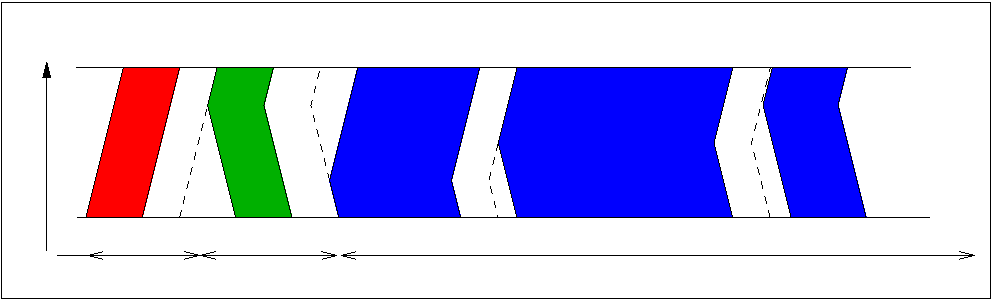
\includegraphics[scale=0.8]{xfig/dorisScenar}
  \input{fig/dorisScenar.pstex_t}
  \caption{Um exemplo de chip \label{fig:dorisScenar}}
\end{figure}


\section{Composi��o dos aneis}

\subsection{Modelo}

Para gerar dinamicamente a composi��o dos dois an�is $\RTS$ e $\SOS$, � preciso
utilizar mecanismos espec�ficos baseados no modelo de falhas adotado
\cite{Lamport84,Cristian95a}.

Neste trabalho, assume-se que os n�meros m�ximos de tarefas e processos s�o
conhecidos antes de inicializar o protocolo \doris{} num segmento.  Denota-se
respectivamente $N^{max}_S$ e $N^{max}_H$ estes n�meros.  Considera-se tamb�m que as
tarefas e os processos admiss�veis nos aneis tem um identificador absoluto �nico.
Este identificador, denotado $id$, � geralmente diferente do indice da tarefa ou
processo no conjunto $\RTS$ e $\SOS$.

Em rela��o ao modelo de falha, assume-se que mensagens podem ser corrompidas ou n�o
emitidas por uma esta��o (omiss�o), mas que a fun��o de sensoriamento do meio pelas
esta��es n�o falha, isto �, o sensoriamento � confi�vel. Isto implica que se uma
mensagem � transmitida no meio f�sico, todas as esta��es, inclusive a esta��o
emissora daquela mensagem, percebem a transmiss�o desta mensagem, mesmo que elas n�o
consigam a processar corretamente.

Podemos expressar este modelo atrav�s das seguintes propriedades:

\begin{itemize}
\item Uma tarefa ou um processo sempre detecta a sua pr�pria falha
  (``self-awareness''),
\item Uma tarefa sempre detecta corretamente a falha de uma outra tarefa.
\end{itemize}

Esta segunda propriedade decorre da periodicidade das mensagens elementares.  J� que
a falha eventual de uma tarefa causa a aus�ncia da mensagem elementar desta tarefa
no seu devido chip, todas as outras tarefas detectam a aus�ncia de mensagem (estado
do meio ``idle'') e inferem a falha da tarefa correspondente.

No caso dos processos, a aus�ncia de uma mensagem pode ser devida a uma falha ou a
aus�ncia de mensagem para ser transmitido por aquele processo. Portanto, outros
processos n�o podem deduzir nada da aus�ncia, mesmo continuamente repetida, de
mensagens de um certo processo.

Esta propriedade do protocolo \doris{} carateriza a independ�ncia entre os dois
an�is, isto �: uma tarefa de $\RTS$ s� conhece a composi��o do anel $\RTS$, mas n�o
conhece a composi��o do anel $\SOS$. Da mesma forma, os processos de $\SOS$ n�o
conhecem a composi��o de $\RTS$.


\subsection{Mecanismo}

O mecanismo de admiss�o de tarefas nos aneis $\RTS$ e $\SOS$ utiliza um \emph{round}
de admiss�o. A sucess�o de seq��ncias de rota��o entre dois \emph{round} de admiss�o
� chamada de ciclo de communica��o.  Num ciclo de comunica��o, o conjunto de tarefas
membros de

Durante um \emph{round} de admiss�o, cada tarefa admiss�vel disponha de um slot,
determinado de maneira �nica atrav�s do seu identificador absoluto, para transmitir
sua inten�ao de pertencer ao pr�ximo grupo de comunica��o. Se uma tarefa $T_{id}$
emite uma mensagem durante o seu slot de admiss�o, a propriedade de sensoriamento
confi�vel implica que todas as tarefas percebem esta mensagem, inclusive a pr�pria
tarefa $T_{id}$. Portanto, todas as tarefas concordam para incluir $T_{id}$ no
pr�ximo grupo de comunica��o constituindo $\RTS$.  Se um slot permanece vazio
durante o \emph{round} de admiss�o, isto signica que a tarefa correspondente n�o
pertencer� ao pr�ximo grupo de comunica��o.  Este mecanismo aproveita ao m�ximo da
sincroniza��o temporal das esta��es, interpretando a omiss�o de uma mensagem num
determinado slot como a aus�ncia da esta��o correspondente para o pr�ximo ciclo de
communica��o.

Para n�o alterar as propriedades

O seq�enciamento dos slots de admiss�es baseia-se no sincronismo da


No entanto, uma tarefa que deixa de emitir duas mensagens elementares em seguida �
removida do anel pelas outras tarefas.  Pela propriedade de sensoriamento confi�vel,
se uma mensagem n�o � transmitida no meio, por exemplo porque uma falha de omiss�o
occoreu, a esta��o que falhou percebe que o seu slot elementar de emiss�o ficou
vazio, portanto ela ``percebe'' a suas proprias falhas e pode se remover do anel de
forma consistente com as demais esta��es.


\section{Observa��es finais}

Uma observa��o deve ser colocada a respeito do nosso modelo determin�stico. Usando
temporizadores, o protocolo de circula��o do bast�o circulante virtual poderia permitir
que uma tarefa de $\RTS$ se omitisse quando ela n�o tiver nada para transmitir e que
o bast�o circulante passasse logo para a pr�xima esta��o, sem espera nenhuma. No entanto,
esta melhoria em termos de efici�ncia (\emph{throughput}) da comunica��o,
introduziria uma variabilidade no tamanho dos chips, sem melhorar o pior caso para
as tarefas com requisitos temporais cr�ticos. Al�m disso, a detec��o de falhas seria
dificultada. Por esta raz�o, o protocolo \doris{} n�o implementa esta op��o. Ou
seja, para garantir a periodicidade exata dos \emph{slots} de comunica��o, o tamanho
$\DDC = \DHW + \DSW$ dos chips � suposto constante. O determinismo introduzido desta
forma facilita a detec��o eficiente das falhas de processos; dado que cada chip de
\doris{} cont�m uma mensagem elementar, a periodicidade do nosso modelo permite
determinar exatamente quando uma mensagem elementar deve ser observada. Portanto, se
no instante previsto, o meio est� livre, isto significa que uma falha de omiss�o ou
de parada ocorreu.  A conseq��ncia do determinismo assim introduzido � um
\textit{overhead} m�ximo de $2 \, \delta$ por chip de \doris{}, isto �
aproximadamente 4,6\% da banda.

O protocolo \doris{} precisa que haja pelo menos uma esta��o cr�tica at�va no anel
$\RTS$ para funcionar.

Em rela��o a toler�ncia a falhas dos canais de comunica��o, a redund�ncia do
barramento f�sico dever� ser considerada ~\cite{Kopetz05,Avizienis04}.


\end{comment}


%\chapter{A disciplina \emph{DoRiS}} % (10 pag)
\label{cap:specVerif}

%\chapter{Plataforma Operacional}
\label{cap:platOp}

%\chapter{Implementa��o}
\label{cap:implementacao}

% \end{spacing}

%%
%% Parte p�s-textual
%%
\backmatter

\label{ap:dorisSpec}
\label{ap:traces}

% Bibliografia
% � aconselh�vel utilizar o BibTeX a partir de um arquivo, digamos "biblio.bib".
% Para ajuda na cria��o do arquivo .bib e utiliza��o do BibTeX, recorra ao
% BibTeXpress em www.cin.ufpe.br/~paguso/bibtexpress
\renewcommand{\bibname}{REFER�NCIAS}
%\nocite{*}
%\bibliographystyle{authordate2}
%\bibliographystyle{abnt-alf}

\bibliography{../../bib}

\label{app:especificacao}
%% Fim do documento
\end{document}
